\documentclass[a4paper,twoside,master.tex]{subfiles}
\begin{document}
\lecture{7}{Wednesday, January 29, 2020}{The Maxwell Boltzmann Distribution}

\section{The Maxwell Boltzmann Distribution}
\label{sec:the_maxwell_boltzmann_distribution}

Start with our microstate:
\begin{equation}
    \Pr(\{\va{q}, \va{p}\}) = \frac{\delta(E - H(q, p))}{N! h^{3N} \underbrace{\Omega(E,V,N)}_{\int \frac{\dd{q} \dd{p}}{h^{3N} N!} \delta(E-H(q, p))}}
\end{equation}

Next, marginalize over all particles except for the first one:
\begin{align}
    \Pr(\va{q}_1, \va{p}_1) &= \int \dd[3]{q_2} \dd[3]{q_3} \cdots \dd[3]{q_N} \dd[3]{p_2} \dd[3]{p_3} \cdots \dd[3]{p_N} \Pr(\{\va{q}, \va{p}\}) \\
    &= \frac{1}{h^{3N} N! \Omega(E,V,N)} \int \dd[3]{q_2} \dd[3]{q_N} \dd[3]{p_2} \cdots \dd[3]{p_N} \delta\left( E - \sum_{j=1}^{N} \frac{\va{p}^2_j}{2m} \right)
\end{align}

Now notice that
\begin{equation}
    \Omega\left( E - \frac{\va{p}_1^2}{2m}, V, N-1 \right) = \frac{1}{h^{3(N-1)} (N-1)!} \int \dd[3]{q_2} \cdots \dd[3]{q_N} \dd[3]{p_2} \cdots \dd[3]{p_N} \delta\left( \overbrace{E - \frac{\va{p}_1^2}{2m} - \underbrace{\sum_{j=2}^{N} \frac{\va{p}_j^2}{2m}}_{H_{N-1}}}^{-H_N} \right)
\end{equation}

Therefore,
\begin{equation}
    \Pr(\va{q}_1, \va{p}_1) = \frac{\Omega\left( E - \frac{\va{p}^2_1}{2m}, V, N-1 \right)}{h^3 N \Omega(E, V, N)}
\end{equation}

We don't actually care about $ \va{q}_1 $, since nothing in this probability distribution depends on it.

\begin{equation}
    \Pr(\va{p}_1) = \frac{V}{h^3 N} \frac{\Omega\left( E - \frac{\va{p}_1^2}{2m}, V, N-1 \right)}{\Omega(E, V, N)}
\end{equation}

Again, we are going to want to maximize this probability to find the most likely microstate, and as usual, it will be easier to maximize the logarithm:
\begin{equation}
    \ln{\Pr(\va{p}_1)} = \underbrace{\ln\left( \Omega \left( E - \frac{\va{p}_1^2}{2m}, V, N-1 \right) \right)}_{\sim \ln{\Omega(E, V, N-1) - \frac{\va{p}_1^2}{2m} \pdv{\ln(\Omega(E, V, N-1))}{E}} + \ldots} + \text{const.}
\end{equation}
Here we are using a Taylor expansion. Let's define
\begin{equation}
    \beta = \pdv{E} \left[ \ln\left\{ \Omega(E, V, N-1) \right\} \right]
\end{equation}
so
\begin{equation}
    \ln{\Pr(\va{p}_1)} = \text{const.} - \beta \frac{\va{p}^2_1}{2m} + \text{ higher order terms}
\end{equation}
Therefore, to good approximation,
\begin{equation}
    \Pr(\va{p}_1) = \text{const.} \times e^{- \beta \va{p}^2_1 / 2m} = \left( \frac{\beta}{2 \pi m} \right)^{3/2} e^{- \beta \frac{\va{p}_1^2}{2m}}
\end{equation}
since the probability distribution must be normalized. Component-wise, we can write
\begin{equation}
    \Pr(p_{1x}) = \sqrt{\frac{\beta}{2 \pi m}} e^{- \beta \frac{p_{1x}^2}{2m}} 
\end{equation}

What does this actually tell us? What is this $ \beta $ factor that we created? Recall that we define the change in momentum as
\begin{equation}
    \Delta p = F \Delta t
\end{equation}
in simple Newtonian mechanics. If we put particles in a box with a wall of area $ A $, over a time scale $ \Delta t $, how many particles will hit the wall, and how much momentum will they impart onto the wall? For any given velocity, there is a maximum distance $ v_x \Delta t $ for which all particles within this distance will hit the wall if the $ x $-component of their velocity is $ v_x $. Particles at that distance which are moving slower will never hit the wall in $ \Delta t $, and particles moving faster will have a greater chance to hit.

\begin{figure}[h]
    \centering
    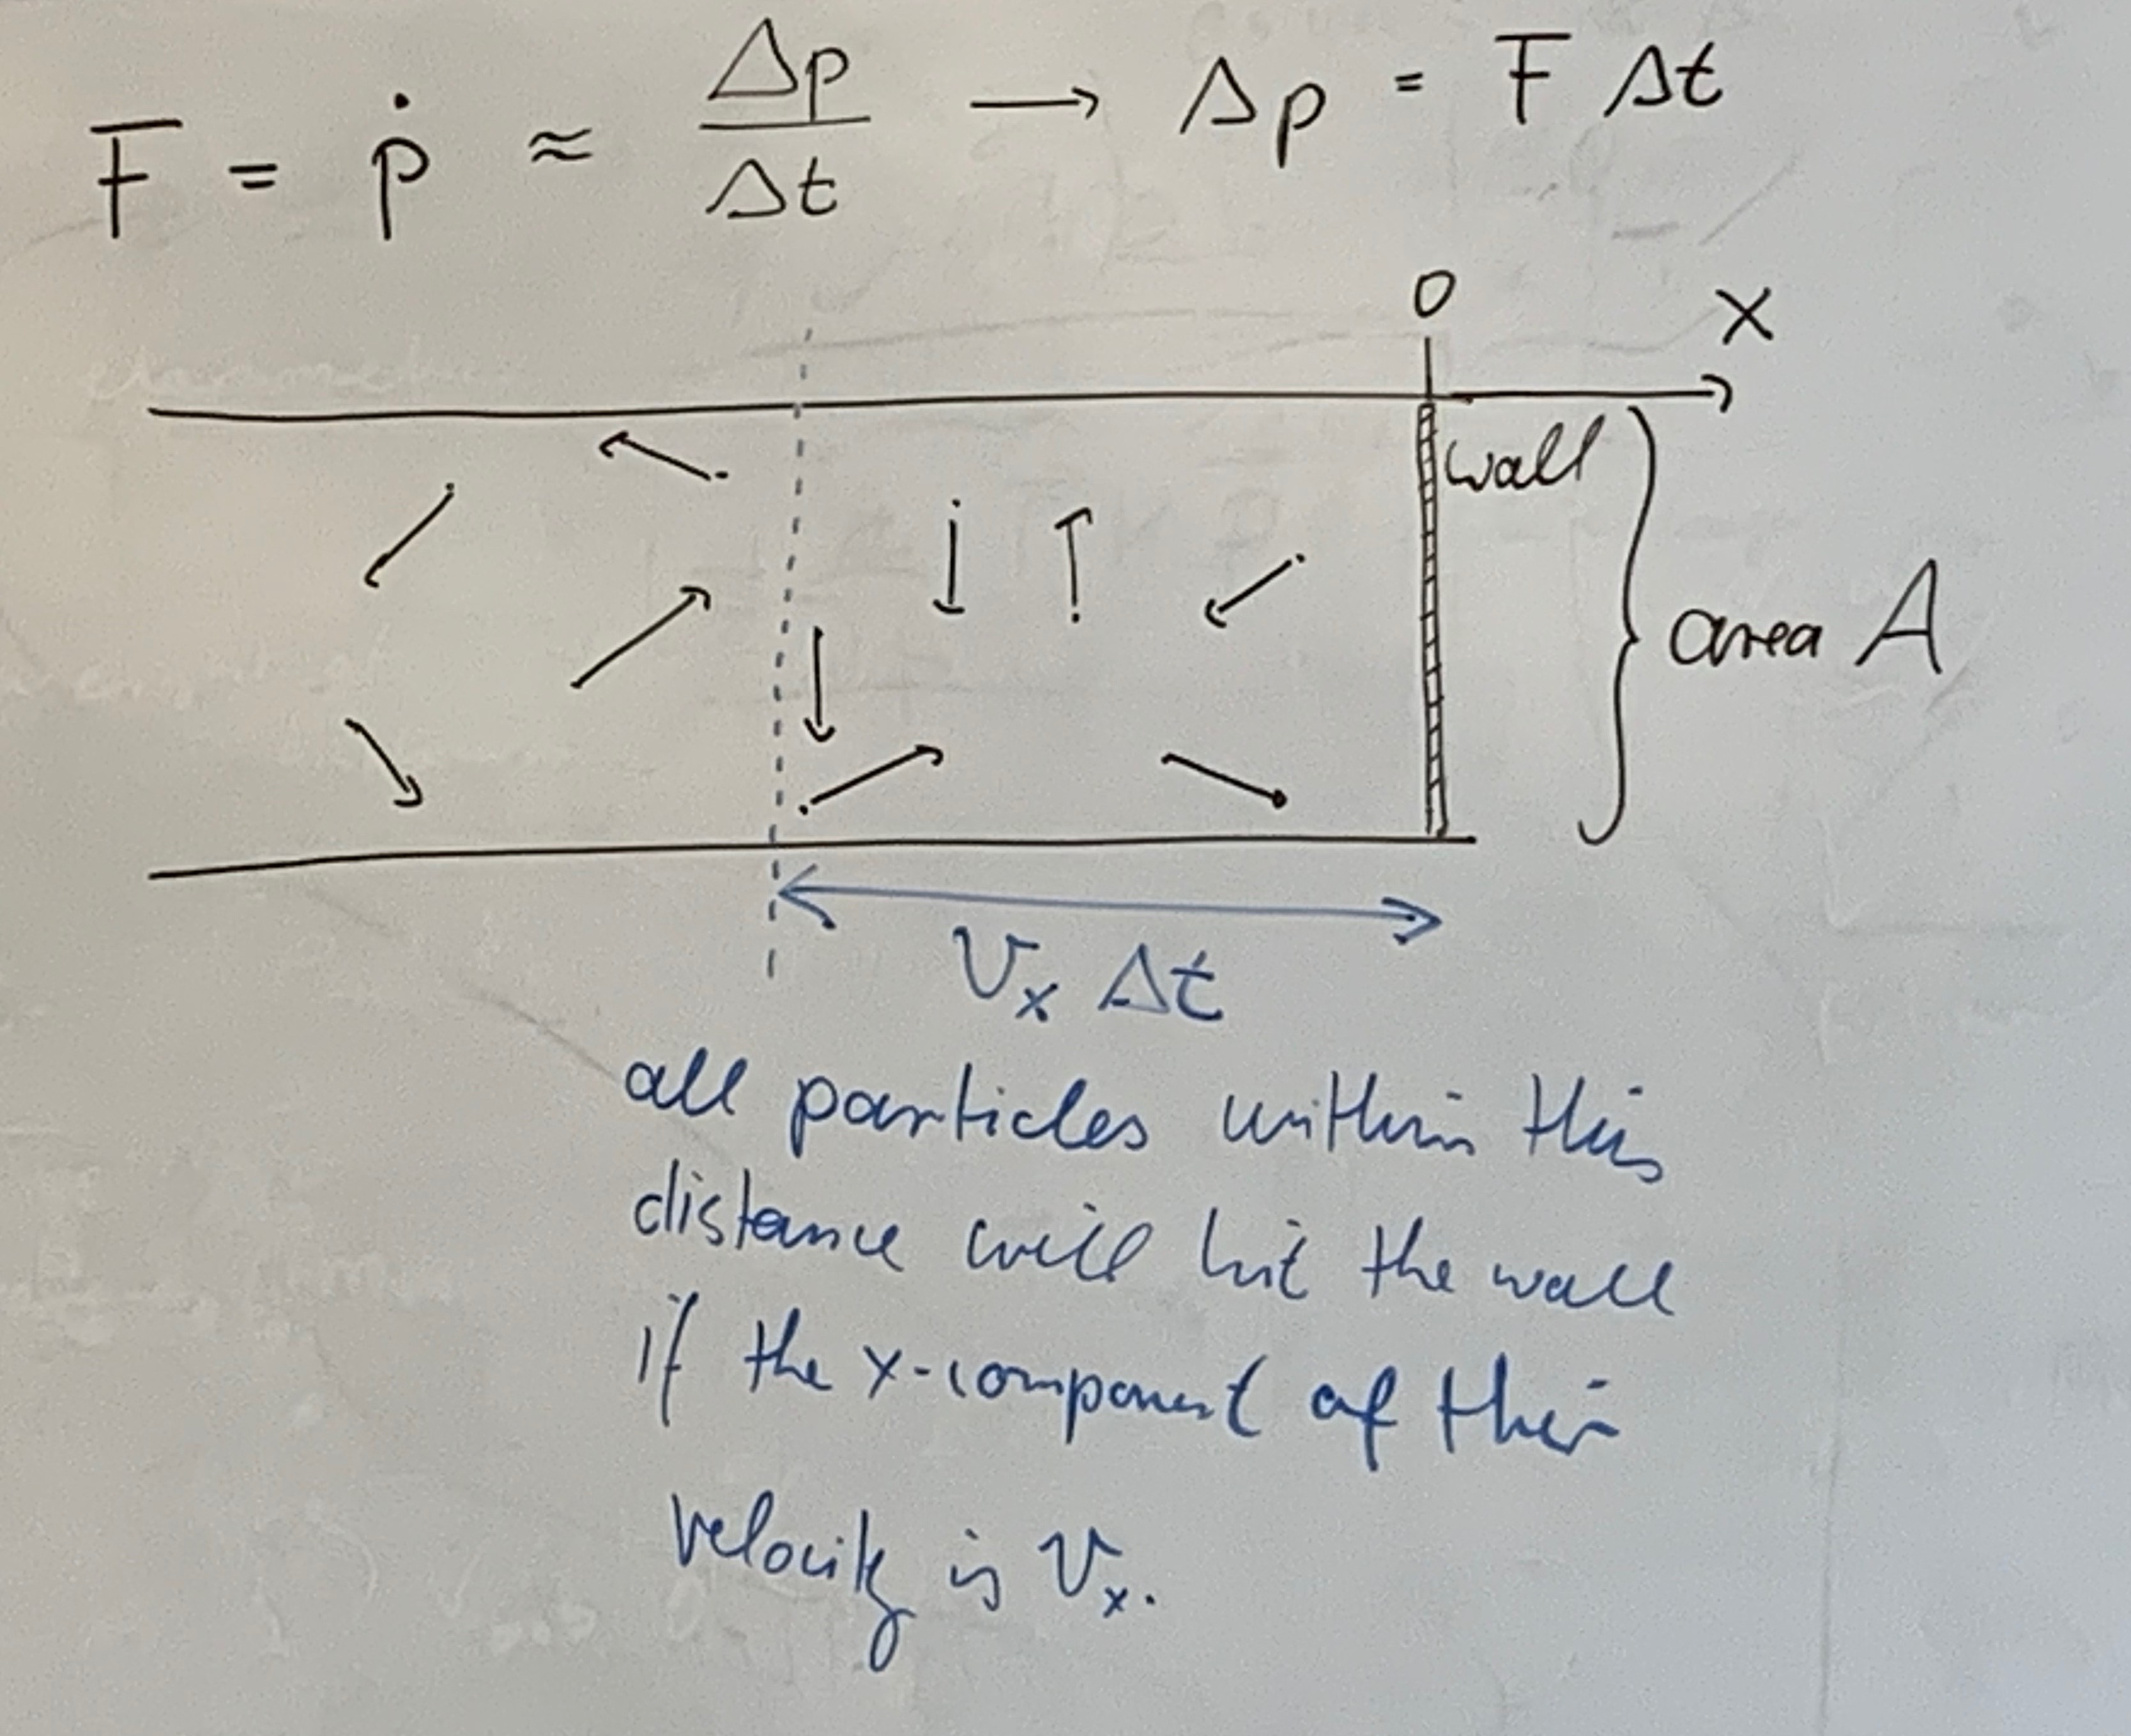
\includegraphics[width=\textwidth/2]{figures/lec_07_pressure_box.png}
    \caption{Pressure on wall with area $ A $}
    \label{fig:lec_07_pressure_box}
\end{figure}

We can write this change as
\begin{equation}
    F \Delta t = \Delta p_x = \int_0^{\infty} \dd{p_x} \left\{\underbrace{\sqrt{\frac{\beta}{2 \pi m}} e^{\beta \frac{p_x^2}{2m}}}_{\parbox{10em}{fraction of particles with momentum within $ p_x $ and $ p_x + \dd{p_x}$}} \times \underbrace{2 p_x}_{\text{momentum exchange}} \times \underbrace{\frac{N}{V} \underbrace{\times A \times \underbrace{\Delta t \times \underbrace{\frac{p_x}{m}}_{v_x}}_{\Delta t v_x = L_x}}_{\text{volume of the hitting particles}}}_{\text{total number of particles in hitting volume}}\right\}
\end{equation}
Evaluating this integral, we find
\begin{equation}
    \Delta p_x = \sqrt{\frac{\beta}{2 \pi m}} 2 \frac{NA}{V} \Delta t \frac{1}{m} \underbrace{\int_0^{\infty} \dd{p_x} p_x^2 e^{- \beta p_x^2 / 2m}}_{\frac{m}{2 \beta} \left( \frac{2 \pi m}{\beta} \right)^{\frac{1}{2}}} = \frac{N}{V} A \Delta t \frac{1}{\beta}
\end{equation}
The pressure is defined as $ P = \frac{F}{A} $ so
\begin{equation}
    P = \frac{N}{V \beta}
\end{equation}

Now let's compare. Our calculation tells us that
\begin{equation}
    PV = \frac{N}{\beta}
\end{equation}
The ideal gas law says that
\begin{equation}
    PV = N k_B T
\end{equation}
Therefore
\begin{equation}
    \beta = \frac{1}{k_B T}
\end{equation}

Let's then go back to entropy:
\begin{equation}
    \pdv{S}{E} = \pdv{E}\left[ k \ln(\Omega(E,V,N)) \right] = k \pdv{E} \left( \ln\left[ \Omega(E, V, \overbrace{N}^{\approx N-1}) \right] \right) = \frac{k}{k_B T} = \frac{1}{T}
\end{equation}
if we allow that $ k $ in the entropy to be the Boltzmann constant. Any other choice in $ k $ just scales the relative temperatures.

Let's look at some other derivatives that we care about. We would expect the derivative of entropy with respect to volume to be the pressure, because if we have a moving wall, the point at which the entropy maximizes is where the pressures equilibrate, so the wall should stop moving and the volumes should also stop changing.

\begin{equation}
    \pdv{S}{V} = \pdv{V} \left\{ k_B N \left[ \frac{3}{2} \ln{\frac{E}{N}} + \ln{\frac{V}{N}} + \text{const.}\right] \right\} = \frac{k_B N}{V} = \frac{P}{T}
\end{equation}
using the ideal gas law $ PV = N k_B T $.

Conversely,
\begin{equation}
    \frac{P}{T} = \pdv{S}{V}
\end{equation}
gives the ideal gas law, so
\begin{equation}
    \frac{1}{T} = \pdv{E}\left\{ k_B N \left[ \frac{3}{2} \ln{\frac{E}{N}} + \ln{\frac{V}{N}} + \text{const.} \right] \right\} = \frac{3}{2} k_B N \frac{1}{E}
\end{equation}
so
\begin{equation}
    E = \frac{3}{2} N k_B T
\end{equation}
This is the ``caloric'' equation of state for a monoatomic ideal gas (as compared to the thermal equation of state\textemdash the ideal gas law).

\end{document}
